\documentclass[a4paper]{report}
\usepackage{amsmath,amsfonts}    % Wiskunde
\usepackage{tikz}

\usepackage{pgfmath}

% Tikz packages
\usetikzlibrary{calc}
\usetikzlibrary{arrows}
\usetikzlibrary{shapes.gates.logic.US}
\usetikzlibrary{shapes.gates.logic.IEC}
\usetikzlibrary{shapes.misc}
\usetikzlibrary{shapes.geometric}
\usetikzlibrary{plotmarks}

% Wiskundige uitdrukkingen voor bv labels
\usepackage{xlop}

\makeatletter
\newcommand{\printresult}[1]{\pgfmathparse{#1}\let\temp@printresult\pgfmathresult\opcopy{\temp@printresult}{a}\opunzero{a}$\opprint{a}$}
\makeatother

\pgfrealjobname{images}

\begin{document}
\beginpgfgraphicnamed{image}
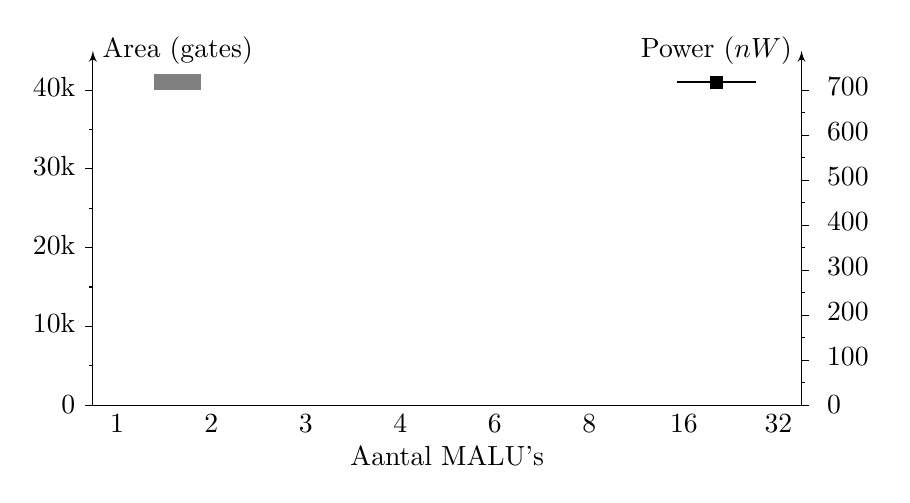
\begin{tikzpicture}
\hspace{-0.5mm}
% Plot area
\begin{scope}[xstep=12mm, x=12mm, ystep=10mm, y=10mm]
	% Data
	\draw [line width=6mm, xshift=3mm + 0.15pt, yshift=0.1pt, color=black!50] plot[ycomb] file{data/results-md-area};
\end{scope}

% Plot power
\begin{scope}[xstep=12mm, x=12mm, ystep=10mm, y=0.05mm]
	% Data
	\draw [xshift=3mm, color=black!90, thick] plot[mark=square*, sharp plot] file{data/results-md-power};
\end{scope}

% Axis
\begin{scope}[xstep=12mm, x=12mm, ystep=10mm, y=10mm]
	% Axis
	\draw [-latex'] (0,0) -- (0,4.5) node[right] (y1) {Area (gates)};
	\draw [-latex'] ($(7, 0) + (6mm, 0)$) -- ++(0, 45mm) node[left] (y2) {Power ($nW$)};
	\draw (0,0) -- node[below, yshift=-4mm] {Aantal MALU's} ($(7, 0) + (6mm, 0)$); 

	% Legende
	\draw [color=black!50, line width=2mm] ($(y1) - (3mm, 4mm)$) -- ++(6mm, 0);
	\draw [thick] ($(y2) - (5mm, 4mm)$) -- plot[mark=square*] coordinates {++(5mm, 0)} -- ++(5mm, 0);

	% Y-axis links
	\draw (-1mm, 0) -- (0, 0) node[left, xshift=-1mm] {0};
	\foreach \y in {1, 2, ..., 4}
		\draw[yshift=\y * 10mm] (-1mm, 0) -- (0, 0) node[left, xshift=-1mm, yshift=0.4mm] {{\printresult{10 * \y}}k};

	\foreach \y in {0, 1, ..., 3}
		\draw[yshift=\y * 10mm + 5mm] (-0.5mm, 0) -- (0, 0);

	% Y-axis rechts
	\draw[xshift=6mm] (7, 0) -- ++(1mm, 0) node[left, xshift=1mm, anchor=west] {0};
	\foreach \y in {10/175, 20/175, 30/175, 40/175, 50/175, 60/175, 70/175}
		\draw[yshift=\y * 100mm, xshift=6mm] (7, 0) -- ++(1mm, 0) node[left, xshift=1mm, yshift=0.4mm, anchor=west] {\printresult{175 * \y}0};

	\foreach \y in {5/175, 15/175, 25/175, 35/175, 45/175, 55/175, 65/175}
		\draw[yshift=\y * 100mm, xshift=6mm] (7, 0) -- ++(0.5mm, 0);

	% X-axis
	\foreach \x / \type in {0 / 1, 1 / 2, 2 / 3, 3 / 4, 4 / 6, 5 / 8, 6 / 16, 7 / 32}
		\draw ($(\x, 0) + (3mm + 0.15pt, 0)$) node[below] {\type};
\end{scope}
\end{tikzpicture}

\endpgfgraphicnamed
\end{document}
